\documentclass[11pt]{article}
\usepackage{amssymb}
\usepackage{amsthm}
\usepackage{enumitem}
\usepackage{amsmath, physics}
\usepackage{bm}
\usepackage{adjustbox}
\usepackage{mathrsfs}
\usepackage{graphicx}
\usepackage{siunitx}
\usepackage[mathscr]{euscript}

\title{\textbf{Solved selected problems of Modern Physics for Scientists and Engineers - John Taylor}}
\author{Franco Zacco}
\date{}

\addtolength{\topmargin}{-3cm}
\addtolength{\textheight}{3cm}

\newcommand{\N}{\mathbb{N}}
\newcommand{\Z}{\mathbb{Z}}
\newcommand{\Q}{\mathbb{Q}}
\newcommand{\R}{\mathbb{R}}
\newcommand{\diam}{\text{diam}}
\newcommand{\cl}{\text{cl}}
\newcommand{\bdry}{\text{bdry}}
\newcommand{\inter}{\text{int}}
\newcommand{\hatx}{\bm{\hat{x}}}
\newcommand{\haty}{\bm{\hat{y}}}
\newcommand{\hatz}{\bm{\hat{z}}}
\newcommand{\hatrho}{\bm{\hat{\rho}}}
\newcommand{\hatphi}{\bm{\hat{\phi}}}
\newcommand{\hatr}{\bm{\hat{r}}}
\newcommand{\hattheta}{\bm{\hat{\theta}}}

\theoremstyle{definition}
\newtheorem*{solution*}{Solution}
\renewcommand*{\proofname}{\bf{Solution}}

\begin{document}
\maketitle
\thispagestyle{empty}

\section*{Chapter 4 - Quantization of Light}

\begin{proof}{\textbf{4.1}}
    We know the Planck distribution function for blackbody radiation is
    \begin{align*}
        I(\lambda, T)
        = \frac{2\pi hc^2}{\lambda^5}\frac{1}{e^{(hc/\lambda k_B T)} -1}
    \end{align*}
    If we take the first factor $2\pi hc^2/\lambda^5$ then as $\lambda \to 0$
    we see that $2\pi hc^2/\lambda^5 \to \infty$ and as $\lambda \to \infty$
    we see that $2\pi hc^2/\lambda^5 \to 0$.\\
    For the second factor we see that as $\lambda \to 0$ we have that
    $1/(e^{(hc/\lambda k_B T)} - 1) \to 0$ and as $\lambda \to \infty$
    we see that $1/(e^{(hc/\lambda k_B T)} - 1) \to \infty$.

    So if we sketch both factors we see in red the factor 
    $1/(e^{(hc/\lambda k_B T)} - 1)$ and in green the factor
    $2\pi hc^2/\lambda^5$.
    \begin{center}
        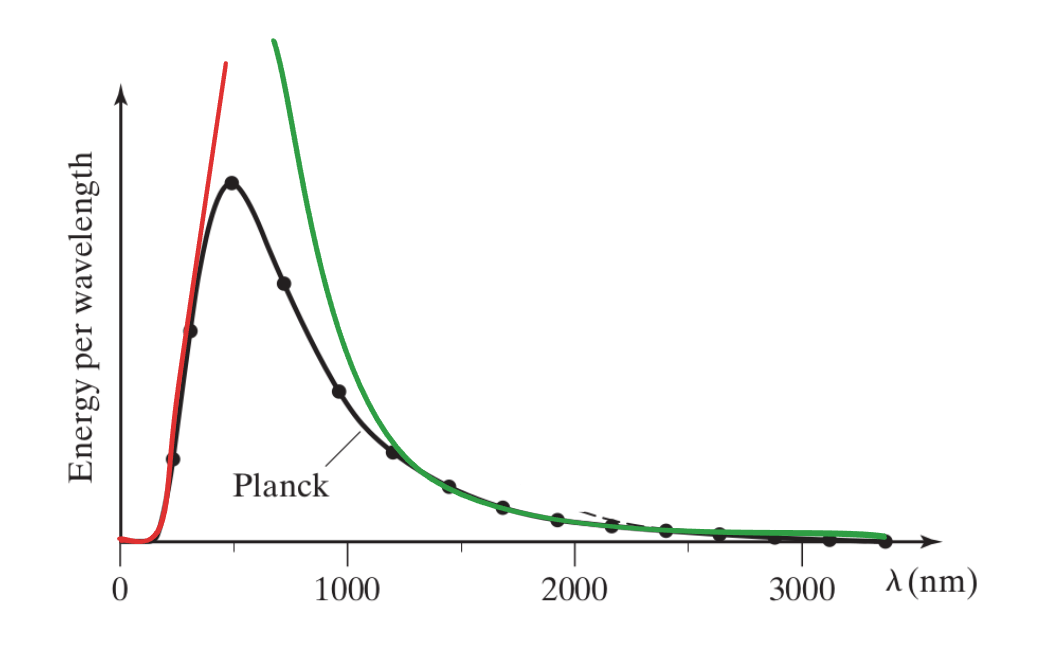
\includegraphics[scale=0.45]{ch4-1.png}
    \end{center}
\end{proof}
\cleardoublepage
\begin{proof}{\textbf{4.2}}
    The Planck formula is given by
    \begin{align*}
        I(\lambda, T)
        = \frac{2\pi hc^2}{\lambda^5}\frac{1}{e^{(hc/\lambda k_B T)} -1}
    \end{align*}
    If we approximate $e^{(hc/\lambda k_B T)}$ by a 2-term Taylor series we
    have that 
    \begin{align*}
        I(\lambda, T)
        &= \frac{2\pi hc^2}{\lambda^5}\frac{1}{1 + \frac{hc}{\lambda k_B T} -1}\\
        &= \frac{2\pi hc^2}{\lambda^5}\frac{\lambda k_B T}{hc}\\
        &= \frac{2\pi c k_B T}{\lambda^4}
    \end{align*}
    Which is the Rayleigh-Jeans distribution function.

    We already have a sketch for the two factors of Plank's formula from
    problem 4.1 adding the sketch for the Rayleigh-Jeans distribution function
    in orange, we see that
    \begin{center}
        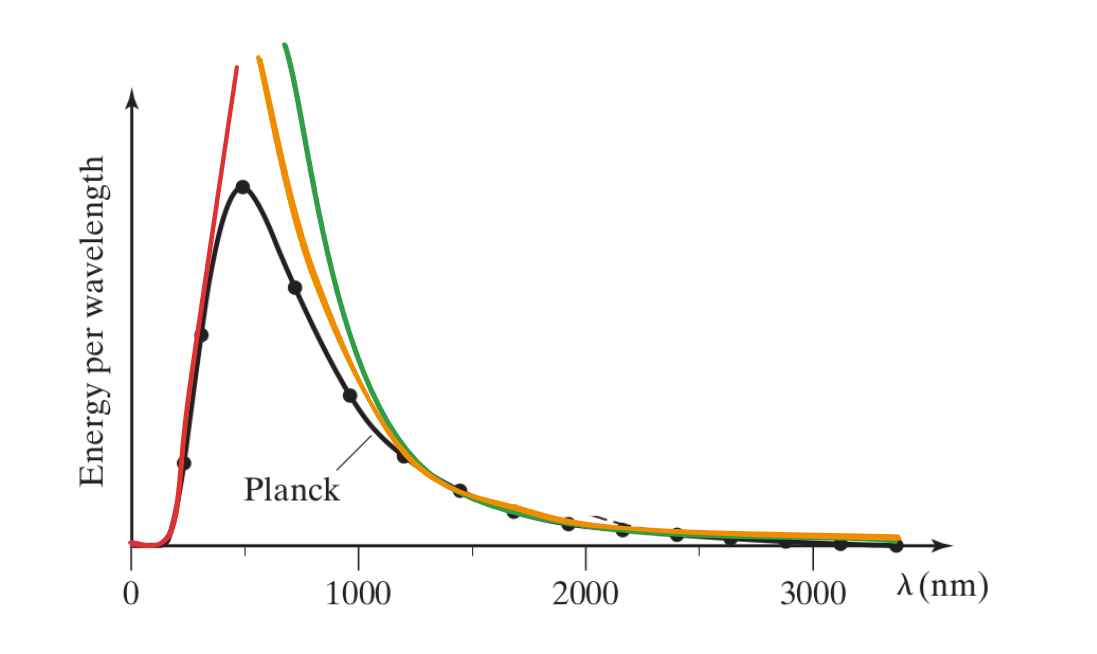
\includegraphics[scale=0.42]{ch4-2.png}
    \end{center}
    Since $2\pi hc^2/\lambda^5$ goes faster to infinity than 
    $2\pi c k_B T / \lambda^4$ as $\lambda \to 0$    

    We might expect the classical result to be better at long wavelength
    since the quantum phenomenons are more notable at smaller scales, and
    they are not so important at long wavelengths.
\end{proof}
\cleardoublepage
\begin{proof}{\textbf{4.3}}
\begin{itemize}
    \item [(a)] We know that the intensity of radiation between $\lambda$
    and $\lambda + d\lambda$ is $I(\lambda, T)d\lambda$.
    If we consider the frequencies related to the wavelength between $\lambda$
    and $\lambda + d\lambda$ the intensity of radiation between $f$ and
    $f + df$ must be $I(f, T)df$ and these intensities must match so
    $I(\lambda, T)d\lambda = I(f, T)df$ therefore must be that
    $$I(f,T) = I(\lambda,T) \bigg|\frac{d\lambda}{df}\bigg|$$
    Where we added the absolute signs to indicate that both distribution
    functions must be positive.
\cleardoublepage
    \item [(b)] We know that the Planck distribution in terms of the wavelength
    is given by
    \begin{align*}
        I(\lambda, T) = \frac{2\pi h c^2}{\lambda^5}
        \frac{1}{e^{hc/\lambda k_B T} - 1}
    \end{align*}
    Also, knowing that $\lambda = c/f$ we have that $d\lambda/df = - c/f^2$.
    Therefore
    \begin{align*}
        I(f, T) &= \frac{2\pi h c^2 f^5}{c^5}
        \frac{1}{e^{hf/k_B T} - 1}~\bigg|\frac{d\lambda}{df}\bigg|\\
        I(f, T) &= \frac{2\pi h f^5}{c^3}
        \frac{1}{e^{hf/k_B T} - 1}~\frac{c}{f^2}\\
        I(f, T) &= \frac{2\pi h f^3}{c^2}
        \frac{1}{e^{hf/k_B T} - 1}
    \end{align*}
    If we take the first factor $2\pi hf^3/c^2$ then as $f \to 0$
    we see that $2\pi hf^3/c^2 \to 0$ and as $f \to \infty$
    we see that $2\pi hf^3/c^2 \to \infty$.\\
    For the second factor we see that as $f \to 0$ we have that
    $1/(e^{(hf/ k_B T)} - 1) \to \infty$ and as $f \to \infty$
    we see that $1/(e^{(hf/ k_B T)} - 1) \to 0$.

    Sketching both factors we see in red the factor 
    $1/(e^{(hf/k_B T)} - 1)$ and in green the factor $2\pi hf^3/c^2$ therefore
    \begin{center}
        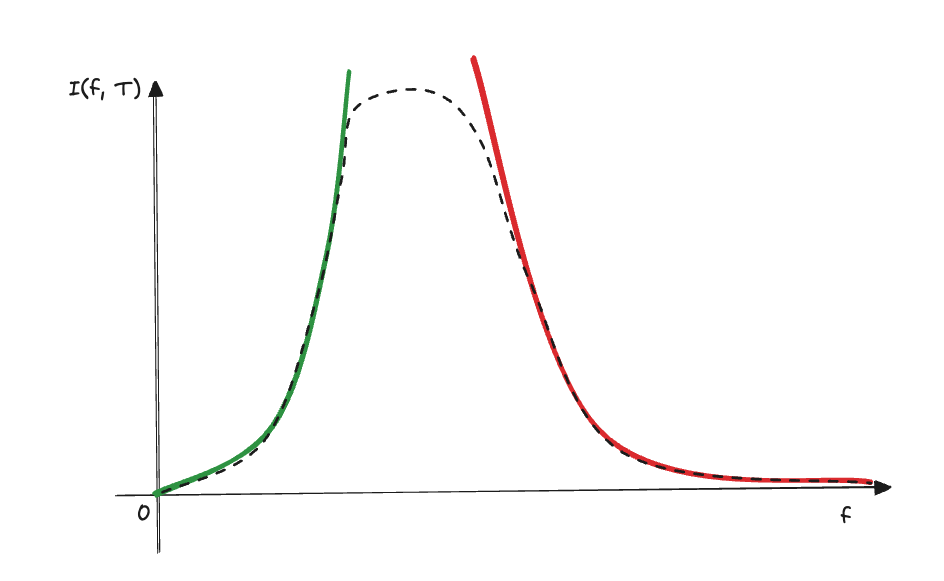
\includegraphics[scale=0.4]{ch4-3.png}
    \end{center}
\end{itemize}
\end{proof}
\cleardoublepage
\begin{proof}{\textbf{4.4}}
\begin{itemize}
    \item [(a)] Let $x = hc/\lambda k_B T$ then from $dx/d\lambda$ we can get
    $d\lambda$ as follows
    \begin{align*}
        \bigg|\frac{dx}{d\lambda}\bigg| &= \frac{hc}{k_B T \lambda^2}\\
        d\lambda &= \frac{k_B T \lambda^2}{hc} dx
    \end{align*}
    By replacing these values we can get total intensity $I(T)$ radiated
    by the following integral
    \begin{align*}
        I(T) &= \int_0^\infty \frac{2\pi h c^2}{\lambda^5}
        \frac{1}{e^{hc/\lambda k_B T} - 1}~d\lambda\\
        &= \int_0^\infty \frac{2\pi h c^2}{\lambda^5}
        \frac{1}{e^{x} - 1}~\frac{k_B T \lambda^2}{hc} dx\\
        &= \int_0^\infty \frac{2\pi c k_B T}{\lambda^3}
        \frac{1}{e^{x} - 1}~\frac{(k_B T)^3}{(k_B T)^3}\frac{(hc)^3}{(hc)^3} dx\\
        &= \int_0^\infty \frac{2\pi c (k_B T)^4x^3}{(hc)^3} 
        \frac{1}{e^{x} - 1}~ dx\\
        &= T^4 \bigg(\int_0^\infty \frac{2\pi k_B^4x^3}{h^3c^2} 
        \frac{1}{e^{x} - 1}~ dx\bigg)
    \end{align*}
    Therefore we see that $I(T)$ has the form $I(T) = \sigma T^4$ where
    $\sigma$ is a constant independent of the temperature.
    
    \item [(b)] Knowing that $\int_0^\infty x^3~dx/(e^x - 1) = \pi^4/15$
    and the result from part (a) we get that the Stephan - Boltzmann constant
    is given by
    \begin{align*}
        \sigma &= \frac{2\pi k_B^4}{h^3c^2} \int_0^\infty 
        \frac{x^3}{e^{x} - 1}~ dx\\
        &= \frac{2\pi^5 k_B^4}{15 h^3c^2}
    \end{align*}

    \item [(c)] Replacing the numerical values of the constants involved in
    the Stephen-Boltzmann constant we get that
    \begin{align*}
        \sigma = \frac{2\pi^5 \cdot (1.38 \times 10^{-23})^4}
        {15 \cdot (6.63 \times 10^{-34})^3 \cdot (2.998 \times 10^8)^2}
        = 5.649 \times 10^{-8} \frac{W}{m^2K^4}
    \end{align*}
    Then the total power radiated by a steel ball of $1~cm$ radius at $1000~K$
    is 
    \begin{align*}
        P = I(1000~K)\cdot A = (5.649 \times 10^{-8}) (1000)^4 (4\pi 0.01^2)
        = 70.987~W
    \end{align*}
\end{itemize}
\end{proof}
\cleardoublepage
\begin{proof}{\textbf{4.5}}
    Given that the visible light has a wavelength between $400~nm$ and $700~nm$
    we have that $1/700 < 1/\lambda < 1/400$ hence by multiplying
    the inequality by $hc = 1240~eV\cdot nm$ we get that
    \begin{align*}
        \frac{1240~eV\cdot nm}{700~nm}
        < \frac{hc}{\lambda}
        < \frac{1240~eV\cdot nm}{400~nm}
    \end{align*}
    Then the range of energies $E = hc/\lambda$ of visible photons is between
    \begin{align*}
        1.77~eV < E < 3.1~eV
    \end{align*}
    Given that UV radiation has shorter wavelength than visible light then UV
    photons will have bigger energies than visible and opposite to this
    since IR radiation has longer wavelength than visible then IR photons
    will have smaller energies than visible.
\end{proof}
\begin{proof}{\textbf{4.9}}
\begin{itemize}
    \item [(a)] For low-intensity microwave radiation with a wavelength of 1cm
    to break a bond in a biological molecule, the photon coming from
    the microwave must have an energy of at least 4eV but a microwave
    photon will have an energy of
    $$E = \frac{hc}{\lambda} = \frac{1240~eV\cdot nm}{1\times 10^7~nm} = 0.000124~eV$$
    Therefore a microwave photon cannot break a biological molecule bond.

    \item [(b)] To break a 4eV bond we need a photon with a wavelength of
    \begin{align*}
        \lambda = \frac{hc}{E} = \frac{1240~eV\cdot nm}{4~eV} = 310~nm
    \end{align*}
    
    \item [(c)] Given that visible light has wavelengths between 400nm and
    700nm then 310nm correspond to UV radiation which has a shorter wavelength.
\end{itemize}
\end{proof}
\cleardoublepage
\begin{proof}{\textbf{4.18}}
    \begin{itemize}
        \item [(a)] Given that the work function for tungsten is $\phi= 4.6~eV$
        the critical frequency below which no electron is emited happens at
        \begin{align*}
            f_0 = \frac{\phi}{h}
            = \frac{4.6~eV}{4.135\times 10^{-15}~eV\cdot s}
            = 1.11 \times 10^{15}~Hz
        \end{align*}
        and this is a critical wavelength of
        \begin{align*}
            \lambda_0 = \frac{c}{f_0}
            = \frac{2.998\times 10^{17}~nm/s}{1.11\times 10^{15}~1/s}
            = 270.1~nm
        \end{align*}
        \item [(b)] If tungsten is irradiated with a photon of wavelength
        $\lambda = 200~nm$ the maximum kinetic energy of the ejected electrons
        is
        $$K_{max} = \frac{hc}{\lambda} - \phi = \frac{1240}{200} - 4.6 = 1.6~eV$$
        \item [(c)] Finally, if tungsten is irradiated with a photon of
        wavelength $\lambda = 300~nm$ the maximum kinetic energy of the ejected
        electrons is
        $$K_{max} = \frac{hc}{\lambda} - \phi = \frac{1240}{300} - 4.6 = -0.46~eV$$
        The negative result implies that a wavelength of 300nm
        is not enough to eject an electron as the critical wavelength is about
        270nm, so to eject an electron we need a photon with a wavelength
        less than or equal to this wavelength.
    \end{itemize}
\end{proof}
\begin{proof}{\textbf{4.19}}
    Let the crystal planes be separated by $d= 0.31~nm$ and let the X-rays
    be of wavelength $\lambda = 0.05~nm$ then by the Bragg law the glancing
    angle $\theta$ is given by
    \begin{align*}
        \theta = \arcsin(\frac{\lambda}{2d})
        = \arcsin(\frac{0.05}{2\cdot 0.31}) = 0.0807~rad = 4.67~deg
    \end{align*}
\end{proof}
\cleardoublepage
\begin{proof}{\textbf{4.21}}
    Given that an X-ray of $\lambda = 0.0438~nm$ gives us three maxima at
    $\theta = 36.7^\circ, 52.8^\circ$ and $84.5^\circ$ then by the Bragg's law
    for the first angle we have that
    \begin{align*}
        2d\sin(36.7^\circ) &= n_1 0.0438\\
        d &= n_1\frac{0.0438}{2\sin(36.7^\circ)}\\
        d &= n_1 0.03664
    \end{align*}
    And for the second and third angle we have that
    \begin{align*}
        d &= n_2\frac{0.0438}{2\sin(52.8^\circ)}\\
        d &= n_2 0.02749
    \end{align*}
    \begin{align*}
        d &= n_3\frac{0.0438}{2\sin(84.5^\circ)}\\
        d &= n_3 0.022
    \end{align*}
    Then making them equal and solving for $n_1/n_2$ and $n_1/n_3$ we get that
    \begin{align*}
        \frac{n_1}{n_2} &= \frac{0.02749}{0.03664} = 0.7502\\
        \frac{n_1}{n_3} &= \frac{0.022}{0.03664} = 0.6004
    \end{align*}
    In the first case, $n_1/n_2$ is close to $3/4$ and in the second
    case $n_1/n_3$ is close to $3/5$ therefore this implies that $n_1 = 3$,
    $n_2 = 4$ and $n_3 = 5$.

    Finally, using Bragg's law for the first angle we get that the spacing
    between crystal planes is
    \begin{align*}
        d &= n_1 0.03664 = 3 \cdot 0.03664 = 0.10992~nm
    \end{align*}
\end{proof}
\cleardoublepage
\begin{proof}{\textbf{4.24}}
    We know that crystals of NaCl have a plane spacing of $d = 0.28~nm$ and
    a monochromatic beam of X-rays is hitting the crystal with a glancing
    angle of $\theta = 20^\circ$. By Bragg's law the wavelength of these
    X-rays is 
    \begin{align*}
        \lambda = 2d\sin\theta = 2\cdot 0.28 \cdot \sin 20^\circ = 0.191~nm
    \end{align*}
    The Duane-Hunt law requires that the electrons' kinetic energy $V_0e$ in
    the X-ray tube must be at least equal to the energy $hf$ of the X-ray
    photons. Therefore we require that 
    \begin{align*}
        V_0e \geq hf = \frac{hc}{\lambda} = \frac{1240~eV\cdot nm}{0.191~nm}
        = 64083.76~eV
    \end{align*}
    or
    \begin{align*}
        V_0 \geq 64083.76~V
    \end{align*}
\end{proof}
\cleardoublepage
\begin{proof}{\textbf{4.28}}
    Let us consider a collision between a photon (with momentum $\bm p_0$ and 
    energy $E_0$) and a stationary free electron.
    \begin{itemize}
    \item [(a)] If the photon bounces back with momentum $\bm{p}$ in
    the direction $-\bm p_0$ and energy $E$, by conservation of energy
    we have that
    \begin{align*}
        E_e + E  &= mc^2 + E_0\\
        \sqrt{(p_ec)^2 + (mc^2)^2} &= mc^2 + E_0 - E 
    \end{align*}
    Where we used that $E_e = \sqrt{(p_ec)^2 + (mc^2)^2}$. Also, by conservation of
    momentum
    \begin{align*}
        \bm{p_e} + \bm{p} &= \bm{p_0}\\
        \bm{p_e} &= \bm{p_0} - \bm{p}        
    \end{align*}
    So
    \begin{align*}
        p_e^2 &= p_0^2 + p^2 + 2p_0p        
    \end{align*}
    Hence since $E_0 = p_0c$ and $E = pc$ we get that
    \begin{align*}
        \sqrt{(p_0^2 + p^2 + 2p_0p)c^2 + (mc^2)^2} &= mc^2 + p_0c - pc \\
        \sqrt{p_0^2 + p^2 + 2p_0p + (mc)^2} &= mc + p_0 - p \\
        p_0^2 + p^2 + 2p_0p + (mc)^2 &= (mc)^2 + 2mc(p_0 - p) + p_0^2 + p^2 - 2p_0p\\
        2p_0p  &= + 2mc(p_0 - p) - 2p_0p\\
        2p_0p  &= + mc(p_0 - p)\\
        2\frac{p_0p}{p_0 - p} &= mc\\
        \frac{p_0 - p}{p_0 p} &= \frac{2}{mc}\\
        \frac{1}{p} - \frac{1}{p_0} &= \frac{2}{mc}
    \end{align*}

    \item [(b)] If we set $\theta = \pi$ in the Compton's fomula we get that
    \begin{align*}
        \frac{1}{p} - \frac{1}{p_0} &= \frac{1}{mc}(1 - \cos\pi)\\
        \frac{1}{p} - \frac{1}{p_0} &= \frac{1}{mc}(1 - (-1))\\
        \frac{1}{p} - \frac{1}{p_0} &= \frac{2}{mc}        
    \end{align*}
    Which is the same result we got.        
    \end{itemize}
\end{proof}
\cleardoublepage
\begin{proof}{\textbf{4.29}}
    Let a 100W beam of light shine for 1000s on a 1g black object initially 
    at rest in a frictionless environment.
    \begin{itemize}
        \item [(a)] Given that the object absorbs all the light produced,
        the total energy absorbed is the energy generated by the beam hence
        \begin{align*}
            E = 100~W \cdot 1000~s = 100000~J % = 6.2415\times 10^{23} ~eV
        \end{align*}
        And therefore the momentum absorbed is 
        \begin{align*}
            p = \frac{E}{c} = \frac{100000~J}{2.998\times 10^8~m/s}
            = 0.0003335~kg\cdot m/s % = 3.335\times 10^{-4}~kg\cdot m/s
        \end{align*}
        \item[(b)] From conservation of momentum we have that
        \begin{align*}
            p_{body} &= p_{beam}\\
            mv &= p_{beam}\\
            v &= \frac{p_{beam}}{m}
        \end{align*}
        Hence
        \begin{align*}
            v &= \frac{0.0003335~kg\cdot m/s}{0.001~kg} = 0.3335~m/s
        \end{align*}
        \item[(c)] The body's final kinetic energy is then
        \begin{align*}
            K &= \frac{1}{2}mv^2\\
            &= \frac{1}{2} \cdot 0.001~kg \cdot (0.3335~m/s)^2\\
            &= 5.5611\times 10^{-5}~J 
        \end{align*}
        This result is a lot less than the 100000J we started from but this is
        because the body is not only transforming the energy into kinetic
        energy but also in kinetic energy on the particles that compose it
        which translate into heat.
        
    \end{itemize}
\end{proof}

\cleardoublepage
\begin{proof}{\textbf{4.32}}
    Below we show a plot of the Plank distribution function for two
    temperatures $T = 1000~K$ and $T = 1500~K$
    \begin{center}
        \includegraphics*[scale=0.7]{ch4-32.png}
    \end{center}
    The curve for $T = 1000~K$ reaches its maximum approximately at
    $\lambda = 2.89~\mu m$ and the curve for $T = 1500~K$ reaches its
    maximum approximately at $\lambda = 1.93~\mu m$.

    The total radiated power is bigger for $T = 1500~K$ since it is
    a function of $T^4$.
\end{proof}
\cleardoublepage
\begin{proof}{\textbf{4.33}}
    We know the Planck distribution function for blackbody radiation is
    \begin{align*}
        I(\lambda, T)
        = \frac{2\pi hc^2}{\lambda^5}\frac{1}{e^{(hc/\lambda k_B T)} -1}
    \end{align*}
    but if we set $x = \lambda k_B T / hc$ we get that
    \begin{align*}
        I(x, T)
        = \frac{2\pi k_B^5 T^5 }{h^4c^3}\frac{1}{x^5}\frac{1}{e^{1/x} -1}
    \end{align*}
    If we derivate this expression using a computer solver we get that
    \begin{align*}
        \derivative{I(x, T)}{x}
        = \frac{2\pi k_B^5 T^5 }{h^4c^3}
        \frac{e^{1/x}(1 - 5x) + 5x}{(e^{1/x}-1)^2x^7}
    \end{align*}
    and making it equal to 0 we get the $x$ where the maximum happens for
    $I(x,T)$ hence
    \begin{align*}
        e^{1/x}(1 - 5x) + 5x &= 0\\
        x_{max} &= 0.201
    \end{align*}
    But $x$ was equal to $\lambda k_B T/hc$ then the value of $\lambda$
    for which $I(\lambda,T)$ is maximum is given by
    \begin{align*}
        \lambda_{max} &= \frac{0.201 hc}{k_B T}
    \end{align*}
    Where we see that $\lambda_{max}$ is proportional to $1/T$ as Wien's 
    displacement law states.
    
    Finally, we do the same analysis but graphically. Let us plot
    $I(x, T)$ and $dI(x,T)/dx$ for $T = 400~K$ then graphically we see that
    \begin{center}
        \includegraphics*[scale=0.7]{ch4-33.png}
    \end{center}
    Where $dI(x,T)/dx$ is 0 approximately at $x = 0.2$ as we saw in the solution
    returned by the computer solver.
\end{proof}


\end{document}
